\documentclass{article}
\usepackage{tikz}
\usetikzlibrary{matrix}

\begin{document}

\begin{figure}[h]
    \centering
    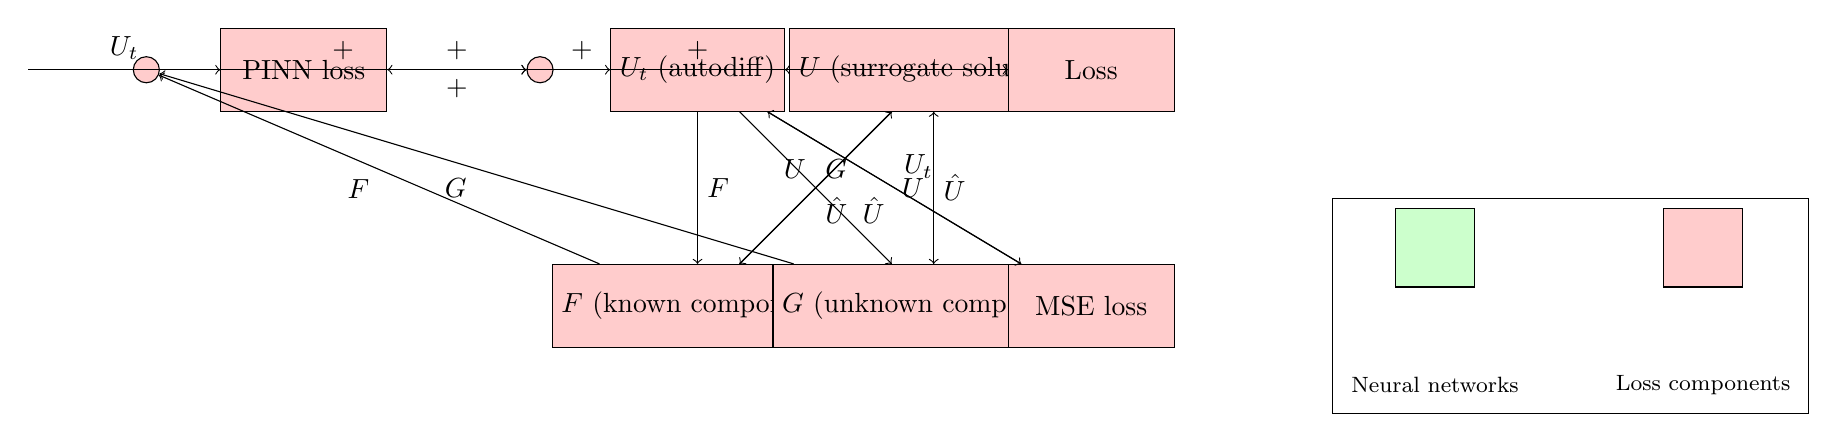
\begin{tikzpicture}[node distance=2cm, auto]
        % Define styles for nodes
        \tikzset{
            block/.style = {draw, fill=red!20, rectangle, minimum height=3em, minimum width=6em},
            sum/.style = {draw, fill=red!20, circle, node distance=1.5cm},
            input/.style = {coordinate},
            output/.style = {coordinate},
            pinstyle/.style = {pin edge={to-,thin,black}}
        }
        
        % Place nodes
        \node [input, name=input] {};
        \node [sum, right of=input] (sum) {};
        \node [block, right of=sum] (controller) {PINN loss};
        \node [sum, right of=controller, node distance=3cm] (sum2) {};
        \node [block, right of=sum2] (system) {$U_t$ (autodiff)};
        \node [block, below of=system, node distance=3cm] (system2) {$F$ (known component)};
        \node [block, right of=system2, node distance=3cm] (system3) {$G$ (unknown component)};
        \node [block, above of=system3, node distance=3cm] (system4) {$U$ (surrogate solution)};
        \node [output, right of=system3] (output) {};
        \node [output, right of=system4] (output2) {};
        \node [block, above of=output, node distance=3cm] (loss) {Loss};
        \node [block, below of=output2, node distance=3cm] (mse) {MSE loss};
        
        % Draw edges
        \draw [->] (input) -- node {$U_t$} (controller);
        \draw [->] (controller) -- node {$+$} (sum2);
        \draw [->] (sum2) -- node {$+$} (system);
        \draw [->] (system) -- node {$F$} (system2);
        \draw [->] (system) -- node {$G$} (system3);
        \draw [->] (system2) -- node {$U$} (system4);
        \draw [->] (system3) -- node {$U$} (system4);
        \draw [->] (system4) -- node {$\hat{U}$} (system3);
        \draw [->] (system4) -- node {$\hat{U}$} (system2);
        \draw [->] (system2) -- node {$F$} (sum);
        \draw [->] (system3) -- node {$G$} (sum);
        \draw [->] (sum) -- node {$+$} (sum2);
        \draw [->] (sum2) -- node {$+$} (controller);
        \draw [->] (controller) -- node {$+$} (loss);
        \draw [->] (loss) -- node {} (system);
        \draw [->] (system) -- node {$U_t$} (mse);
        \draw [->] (mse) -- node {$\hat{U}$} (system);
        
        % Legend
        \matrix [draw, fill=white, matrix of nodes, column sep=1cm, row sep=1cm, right of=mse, anchor=west] at (mse.east) {
            \node[fill=green!20, draw, minimum size=1cm] {}; & \node[fill=red!20, draw, minimum size=1cm] {}; \\
            \node[anchor=center] {\footnotesize Neural networks}; & \node[anchor=center] {\footnotesize Loss components}; \\
        };
    \end{tikzpicture}
    \caption{Overview of the structure of the UPINN method as applied to~\eqref{eq:1}, which shows inputs and outputs of all known and unknown components, as well as losses. The surrogate solution $U$ outputted by the UPINN takes time $t$ as input. Both $F$ (the known component of the differential equation) and $G$ (the unknown component, to be fit by the UPINN) take in time and $\hat{U}$, the prediction of the neural network, as input. $F$ and $G$, along with $U_t$ (the autodifferentiated derivative of $U_{NN}$ w.r.t. time) and is passed as input to the PINN loss. Then, the PINN loss computes the error between $U_t$ and $F+G$. The MSE loss computes the error between the surrogate solution $\hat{U}$ and the data.}
    \label{fig:upinn_structure}
\end{figure}

\end{document}